\documentclass[12pt, letterpaper]{article}
%\documentclass[12pt, letterpaper, titlepage]{article}

\usepackage{amsmath}
\usepackage{booktabs}
\usepackage{amsthm}
\usepackage{graphicx}
\usepackage[margin=1in]{geometry}
\usepackage{hyperref}
\hypersetup{colorlinks = true, linkcolor = blue, citecolor=blue, urlcolor = blue}
\usepackage{enumitem}
\usepackage{setspace}
\usepackage{lipsum}
\usepackage[square,numbers]{natbib}
\bibliographystyle{abbrvnat}



\usepackage[]{lineno}
\linenumbers*[1]
% %% patches to make lineno work better with amsmath
\newcommand*\patchAmsMathEnvironmentForLineno[1]{%
 \expandafter\let\csname old#1\expandafter\endcsname\csname #1\endcsname
 \expandafter\let\csname oldend#1\expandafter\endcsname\csname end#1\endcsname
 \renewenvironment{#1}%
 {\linenomath\csname old#1\endcsname}%
 {\csname oldend#1\endcsname\endlinenomath}}%
\newcommand*\patchBothAmsMathEnvironmentsForLineno[1]{%
 \patchAmsMathEnvironmentForLineno{#1}%
 \patchAmsMathEnvironmentForLineno{#1*}}%

\AtBeginDocument{%
 \patchBothAmsMathEnvironmentsForLineno{equation}%
 \patchBothAmsMathEnvironmentsForLineno{align}%
 \patchBothAmsMathEnvironmentsForLineno{flalign}%
 \patchBothAmsMathEnvironmentsForLineno{alignat}%
 \patchBothAmsMathEnvironmentsForLineno{gather}%
 \patchBothAmsMathEnvironmentsForLineno{multline}%
}

% control floats
\renewcommand\floatpagefraction{.9}
\renewcommand\topfraction{.9}
\renewcommand\bottomfraction{.9}
\renewcommand\textfraction{.1}
\setcounter{totalnumber}{50}
\setcounter{topnumber}{50}
\setcounter{bottomnumber}{50}

\newcommand{\jy}[1]{\textcolor{blue}{JY: #1}}
\newcommand{\eds}[1]{\textcolor{red}{EDS: (#1)}}

% NOTE: To produce blinded version, replace "0" with "1" below.
\newcommand{\blind}{0}


%\title{On Misuses of the Kolmogorov--Smirnov Test for One-Sample Goodness-of-Fit}
%
%\author{Anthony Zeimbekakis\\
%%   \href{mailto:anthony.zeimbekakis@uconn.edu}
%% {\nolinkurl{anthony.zeimbekakis@uconn.edu}}\\
  %Elizabeth D.  Schifano\\
  %Jun Yan\\[1ex]
  %Department of Statistics, University of Connecticut\\
%}
%\date{}

\begin{document}
%\maketitle

\if0\blind
{
  \title{\bf Practicing LaTex/BibTex Assignment}
  \author{Zoe Macris\\[1ex]
%   \href{mailto:zoe.macris@uconn.edu}
% {\nolinkurl{zoe.macris@uconn.edu}}\\
  Department of Statistics, University of Connecticut\\
}
\date{}
  \maketitle} 


\doublespace

\begin{abstract}
This is the abstract. 
\lipsum[1]
\end{abstract}

%\doublespace

\section{Introduction}
\label{sec:intro}

This is the introduction of this sample LaTeX project.
\lipsum[1-2]
Here is example of in-Display equation:
\begin{equation} 
\label{eq1}
\chi ^{2}=\sum\frac{(A-E)^2}{E}\\=\sum^{K}_{1}\frac{(A_{i}-E_{i})^2}{E_{i}}=\sum^{K}_{1}\frac{(A_{i}-np_{i})^2}{np_{i}}
\end{equation}
\lipsum[1-2]
In Section~\ref{sec:fitted}, there will be an example of references. Section~\ref{sec:dependence} will be the example of table and figure. Section~\ref{sec:fittedwithdependence} will have two in line math equations and the last in display equation, just like with this example of reference for in display equation ~\eqref{eq1}. Then there will be an Appendix~\ref{sec:appendix}. 


\section{Reference Examples}
\label{sec:fitted}

\lipsum[1-2]

This is an example of reference with parenthetical citation \citep{example1}.
Whereas \citet{example2} is a good example of reference with textual citation. 


\section{Table and Figure}
\label{sec:dependence}

Below here is an example of a table and a figure. 
\lipsum[1]

\begin{center}
\label{tab:exampletable}
\begin{tabular}{||c c c c||} 
 \hline
 Col1 & Col2 & Col2 & Col3 \\ [0.5ex] 
 \hline\hline
 1 & 5 & 100 & 36912 \\ 
 \hline
 2 & 15 & 150 & 69123 \\
 \hline
 3 & 25 & 200 & 91236 \\
 \hline
 4 & 35 & 250 & 12369 \\
 \hline
 5 & 45 & 300 & 23691 \\ [1ex] 
 \hline
\end{tabular}
\end{center}

\begin{figure}[tbp]
\label{fig:examplefig}
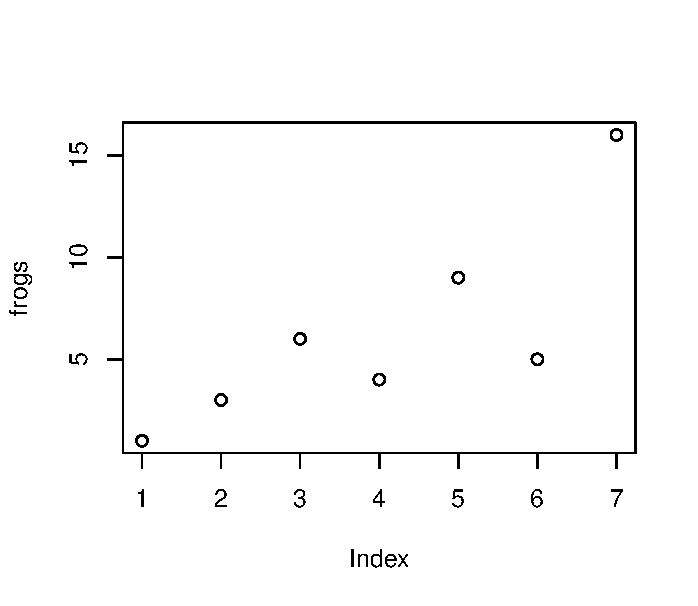
\includegraphics[width=8cm]{examplefigfrog.pdf}
\centering
\end{figure}

The figure ~\ref{fig:examplefig} is a good example of a figure. 
\lipsum[1]
The table ~\ref{tab:exampletable} is a good example of a table. 


\section{Math Equations}
\label{sec:fittedwithdependence}

An example of a math equation within text is \(E=mc^2\). Whereas another in display math equation is:
\begin{equation} \label{eq2}
	\begin{split}
	A & = \frac{\pi r^2}{2} \\
	 & = \frac{1}{2} \pi r^2
\end{split}
\end{equation}
Another example of in text math equation is \(sin^2(a)+\cos^2(a) = 1\). 
\lipsum[1]
We can refer back to in display equations like this ~\eqref{eq2}.

\appendix

\section{Appendix}
\label{sec:appendix}

This is the appendix.
\lipsum[1]


\bibliography{Citations}

\end{document}
%%% LocalWords: nonparametric semiparametric autocorrelation ARMA
%%% Local Variables:
%%% mode: latex
%%% TeX-master: t
%%% ispell-personal-dictionary: ".aspell.en.pws"
%%% fill-column: 80
%%% eval: (auto-fill-mode 1)
%%% End:
